\documentclass{beamer}
\usetheme{metropolis}
\usepackage{amsmath}
\usepackage{pifont}
\usepackage[T1]{fontenc}
\usepackage[font=small,labelfont=bf]{caption}
\fontfamily{verdana}\selectfont
\setlength{\unitlength}{\textwidth}  % measure in textwidths
\setbeamercolor{item}{fg=black}
\setbeamertemplate{itemize items}[triangle] % if you want a ball
\setbeamertemplate{itemize subitem}[triangle] % if you want a circle
\setbeamertemplate{itemize subsubitem}[triangle] % if you want a triangle
\newcommand{\code}[1]{{\texttt{#1}}}

%************ Title & Author ***********************
\title{MSE in a nutshell}
\subtitle{[subtitle]}
\author{[author] \\ \normalfont {\scriptsize \href{mailto:jdoe@doe.com}{<[email]>}}}
\institute{[affiliation]}
\subject{Fisheries Management}
\begin{document}

%*******************************************
\begin{frame}
\titlepage

\end{frame}

%*******************************************
\begin{frame}
\frametitle{Fisheries management}

\centering
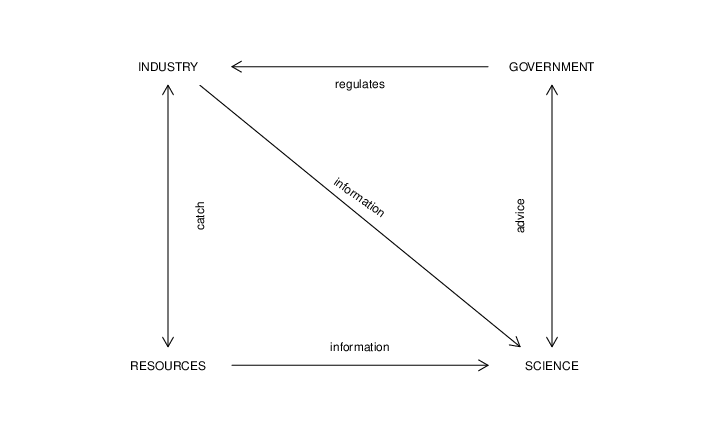
\includegraphics[height=0.8\textheight]{figs/fmanag}

\end{frame}

%*******************************************
\begin{frame}
\frametitle{Goals of fisheries management}

\begin{itemize}
  \item Goals
  \begin{itemize}
    \item Sustainable benefits from harvesting
    \item Conserve stock(s) productivity
    \item Minimise impacts on ecosystem
  \end{itemize}
 \bigskip
    \item Requirements
  \begin{itemize}
    \item Set of clear management objectives
    \item Indication of proper harvest and/or stock level
    \item Means to monitor status
    \item Measures to control fishing
  \end{itemize}
\end{itemize}

\end{frame}

%*******************************************
\begin{frame}
\frametitle{Challenges of fisheries management}

\begin{itemize}
  \item Objectives set to be operational
  \item Trade-offs between short and long term
  \item Monitoring impact to ecosystem
  \item Quantifying uncertainty in status and dynamics
  \item Making decisions acknowledging risks
\end{itemize}

\end{frame}

%*******************************************
\begin{frame}
\frametitle{How to deal with all this? MSE}

\emph{Evaluate the consequences of a range of different management strategies to determine which one will be the most appropriate to meet the operational objectives of the fishery. By:}

\begin{itemize}
	\item Testing how robust the management options are against uncertainty.
    \item Comparing the relative performance of alternative management options.
    \item Simulation-testing management options under a wide(r) range of possible states of nature.
\end{itemize}

\end{frame}

%*******************************************
\begin{frame}
\frametitle{Where does this come from?}

\begin{itemize}	
	\item The International Whaling Commission developed simulation-based management methods using Management Strategies Evaluation (MSE), leading to the Revised Management Procedure (RMP) approved in 1994.
	\item The Revised Management Procedure (RMP) applies MSE to test different whale hunting strategies through simulations before using them in real-world management.
	\item These MSE-based methods account for uncertainty in whale populations and data quality to protect whale stocks through transparent, science-based decisions.
\end{itemize}

\end{frame}

%*******************************************
\begin{frame}
	\frametitle{The RMP}

\centering
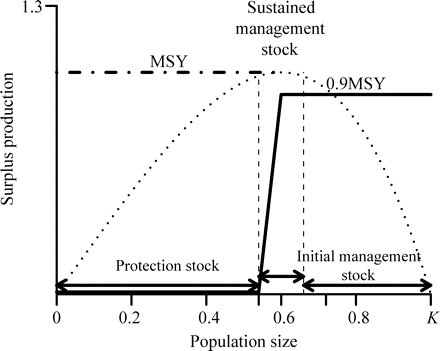
\includegraphics[height=0.7\textheight]{figs/nmp}
	
\end{frame}

%*******************************************
\begin{frame}
\frametitle{IWC: Uncertainties in RMP\footnote{https://iwc.int/rmp2, https://doi.org/10.1093/icesjms/fsm035}}

\begin{itemize}	
	\item Alternative population models.
	\item Initial population size from 5-99% of unexploited (initial, pre-whaling).
	\item Rates of productivity and changes over time.
	\item Uncertainty and bias in the estimated population size.
	\item Frequencies of abundance surveys (every 1, 5 or 10 years).
	\item Changes in carrying capacity (climate change, habitat degradation).
	\item Errors in historic records of catches.
	\item Occurrence of catastrophes (major disease).
	\item Uncertainty about stock structure.
\end{itemize}

\end{frame}

%*******************************************
\begin{frame}
\frametitle{MSE - some examples}

\begin{itemize}	
	\item South African pelagics
	\item Australian fisheries
	\item Commission for the Conservation of Southern Bluefin Tuna
	\item European multi-stocks and multi-gear Management Plans
	\item North Sea Demersals Management Plans
	\item ICCAT ...
	\item IOTC ...
\end{itemize}

\end{frame}

%*******************************************
\begin{frame}
\frametitle{A model of the fishery system}

\begin{center}
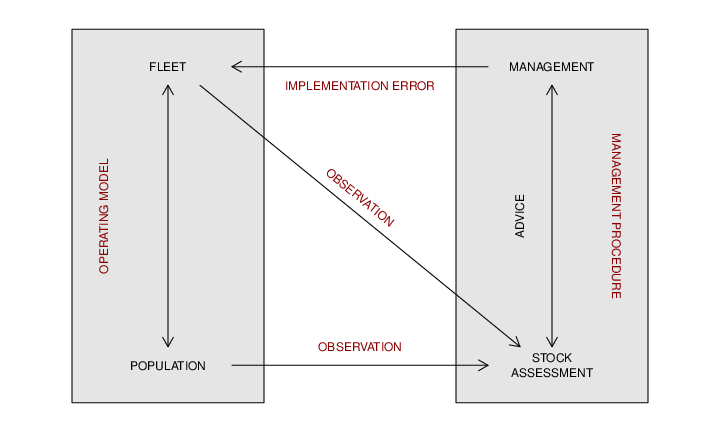
\includegraphics[height=0.8\textheight]{figs/mse.png}
\end{center}

\end{frame}

%*******************************************
\begin{frame}
\frametitle{Six steps to MSE\footnote{Punt, A. E., Butterworth, D. S., de, Moor, C. L., De Oliveira, J. A. and Haddon, M. (2016), Management strategy evaluation: best practices. Fish Fish, 17: 303-334. doi:10.1111/faf.12104}}

\begin{enumerate}	
	\item Define and agree on objectives \& limits
	\item Identify appropriate Management Procedures
	\item Define a set of Operating Models
	\item Conduct simulations
	\item Summarize performance
	\item Select best Management Procedure
\end{enumerate}

\end{frame}

%*******************************************
\begin{frame}
\frametitle{Define objectives \& limits}

IOTC example: 
\begin{itemize}	
	\item objective = $B_{MSY}$, 
	\item limit = $0.40\cdot B_{MSY}$ \& $P(Green) > 60\%$, over next 20
years.
\end{itemize}	

\vspace{1em}

\centering
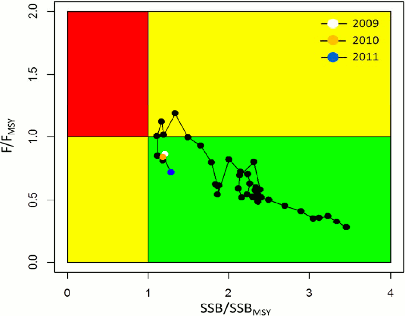
\includegraphics[height=0.5\textheight]{figs/kobe.png}

\end{frame}

%*******************************************
\begin{frame}
\frametitle{Identify Management Procedures}

\begin{enumerate}
	
	\item 
	\begin{minipage}[c]{0.7\textwidth} % Text block
		Observations
	\end{minipage}%
	\hfill
	\begin{minipage}[c]{0.75\textwidth} % Image block
		\centering
		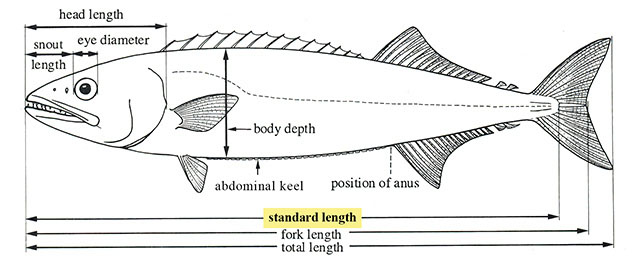
\includegraphics[height=0.18\textheight]{figs/sample}
	\end{minipage}

\bigskip

	\item Estimator of stock status
		\begin{itemize}
			\item stock assessment model, \emph{e.g.} ss3, spict, a4a
			\item or model-free indicator, \emph{e.g.} survey index, CPUE
			\item or data-poor indicator, \emph{e.g.} mean length in the catch 
		\end{itemize}
	
\bigskip

	\item 
	\begin{minipage}[c]{0.7\textwidth}
		Decision
	\end{minipage}%
	\hfill
	\begin{minipage}[c]{0.75\textwidth}
		\centering
		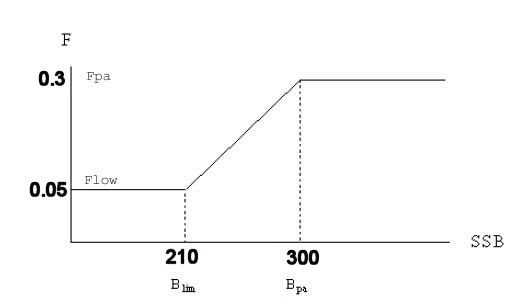
\includegraphics[height=0.25\textheight]{figs/hcr.png}
	\end{minipage}
	
\end{enumerate}

\end{frame}

%*******************************************
\begin{frame}
\frametitle{Define Operating Models}

\centering
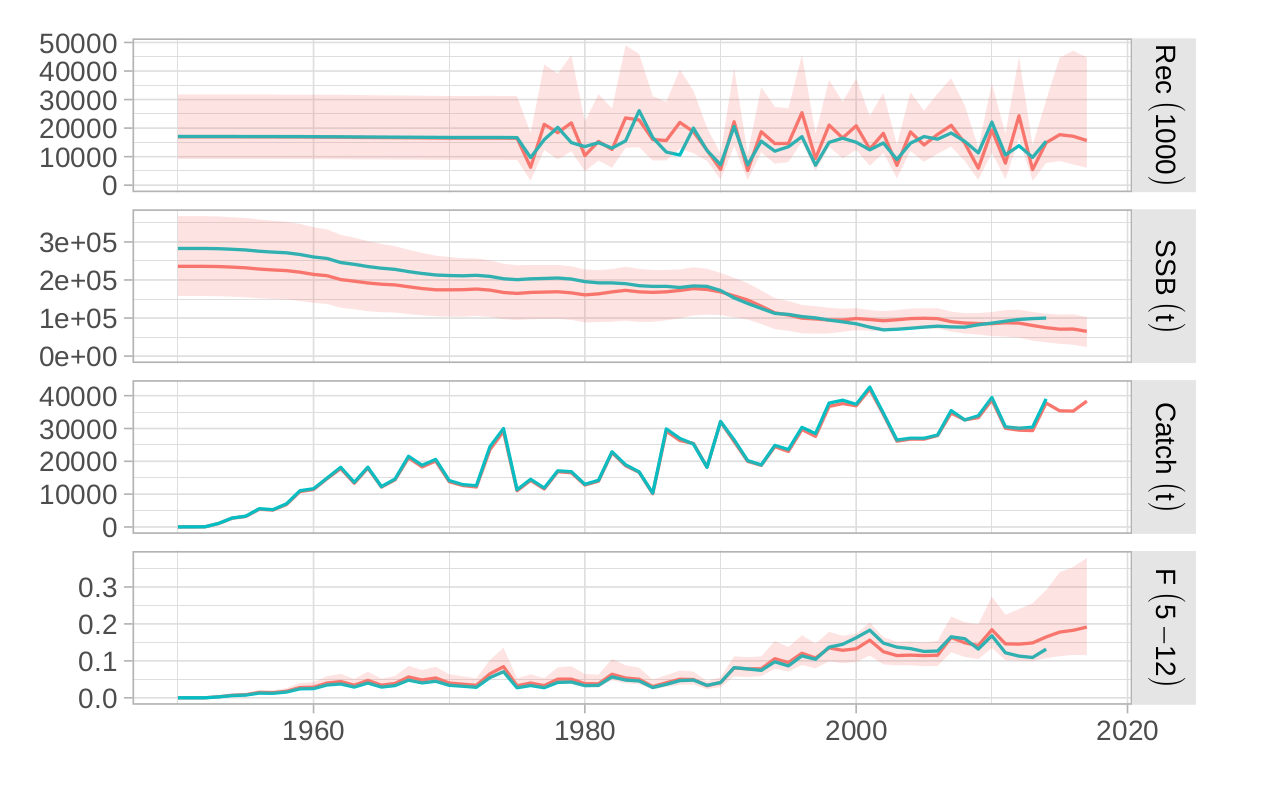
\includegraphics[height=0.8\textheight]{figs/om.png}

\end{frame}

%*******************************************
\begin{frame}
\frametitle{Conduct simulations}

\centering
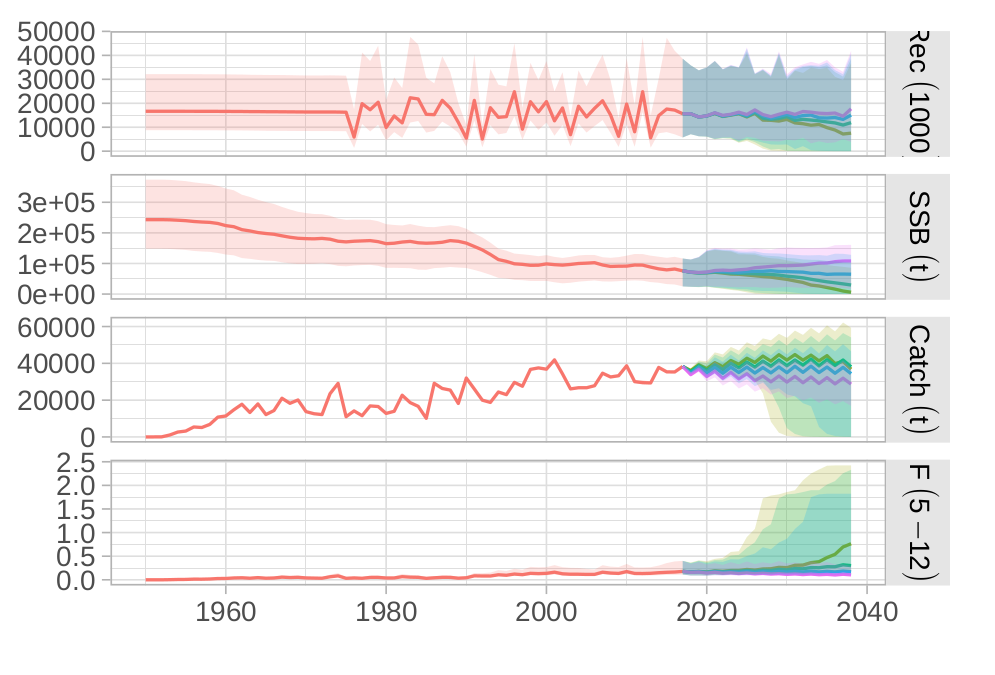
\includegraphics[height=0.8\textheight]{figs/runs.png}

\end{frame}

%*******************************************
\begin{frame}
	\frametitle{Summarize Performance}
	
	\begin{columns}[c] % Vertically center both images
		
		\begin{column}{0.5\textwidth}
			\centering
			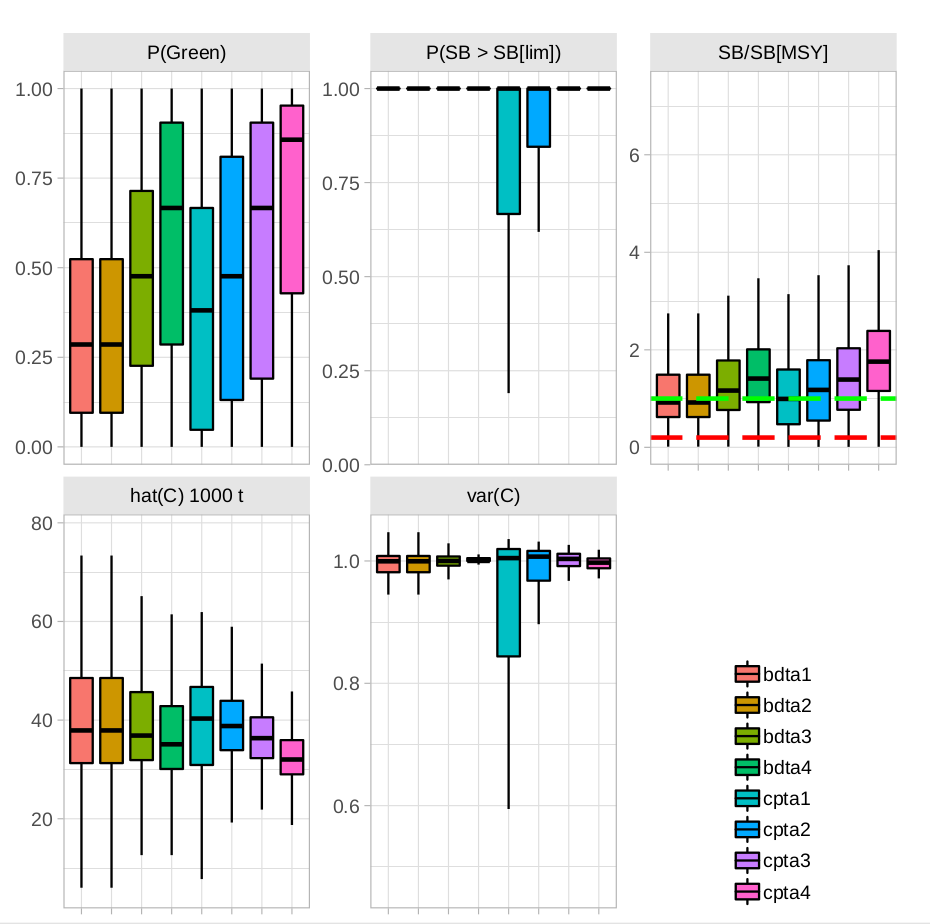
\includegraphics[height=0.7\textheight]{figs/perf1.png}
		\end{column}
		
		\begin{column}{0.5\textwidth}
			\centering
			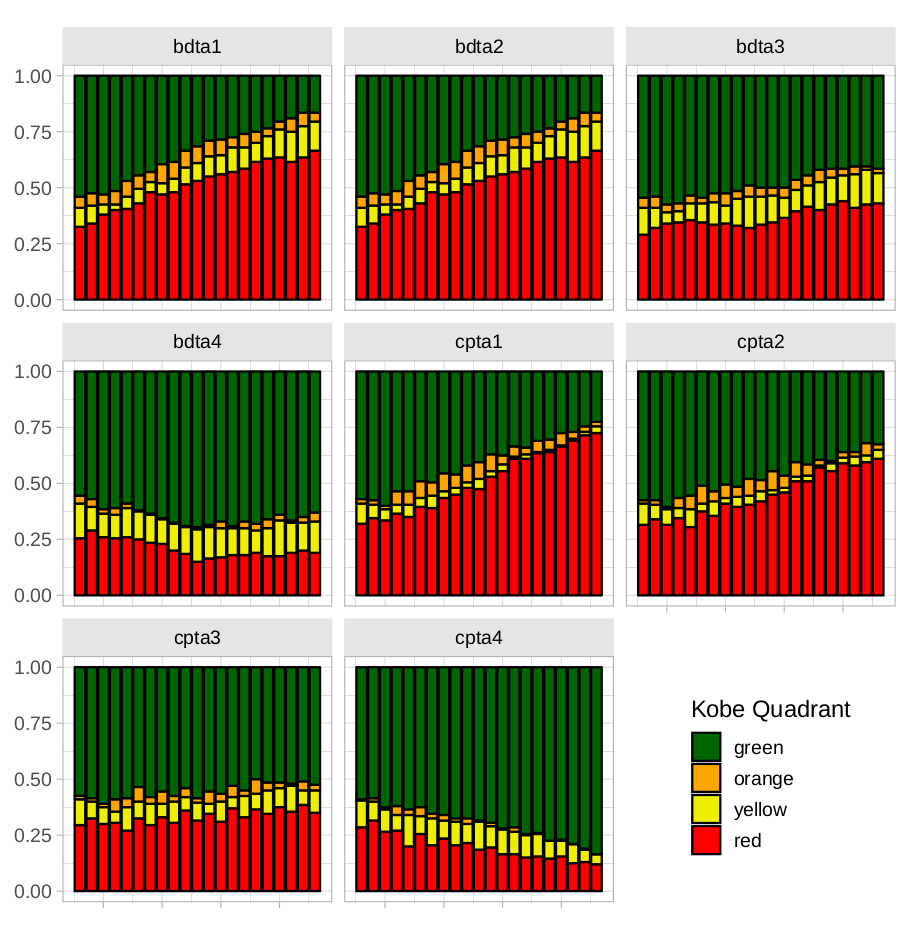
\includegraphics[height=0.7\textheight]{figs/perf2.png}
		\end{column}
		
	\end{columns}
	
\end{frame}

%*******************************************
\begin{frame}
\frametitle{Select best MP}

\begin{center}
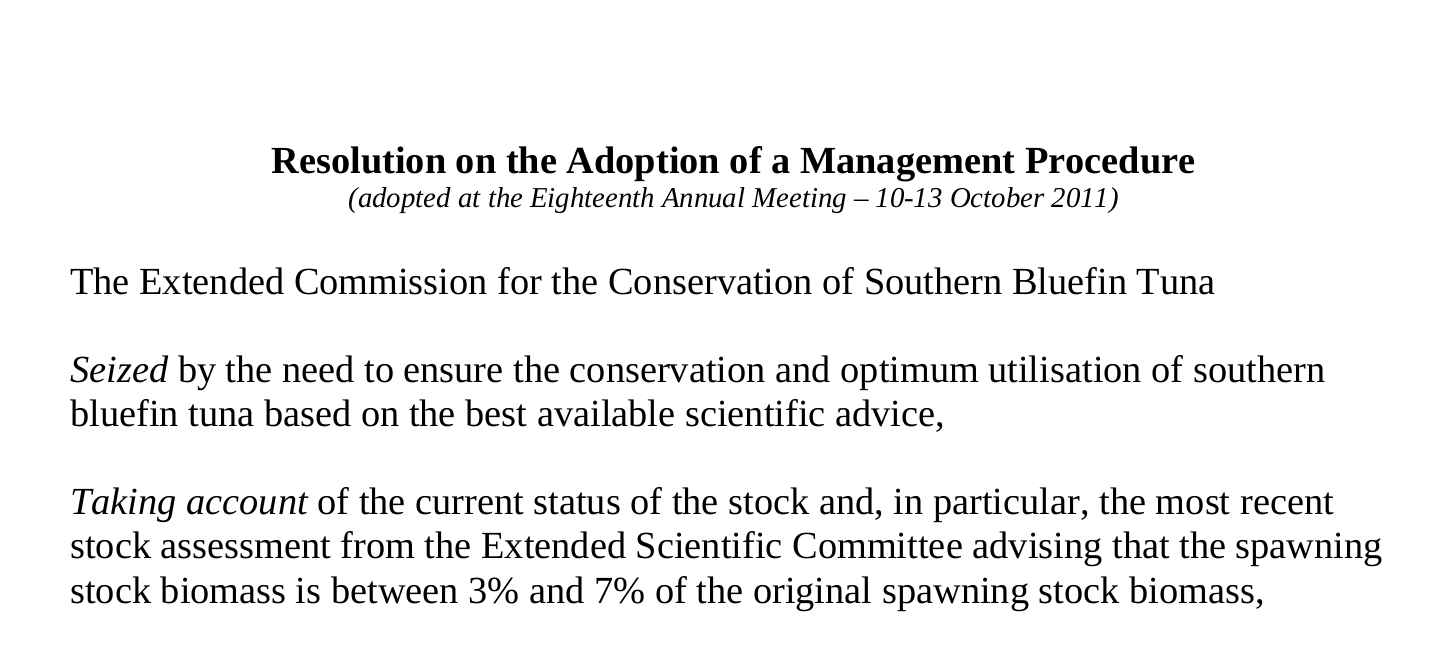
\includegraphics[height=0.6\textheight]{figs/mp.png}
\end{center}

\end{frame}

%*******************************************
% This slide can be used instead of the 4 slides with one advantage in each
\begin{frame}
	\frametitle{What are the advantages?}
	
	\begin{enumerate}
		\item Explicitly Accounts for Uncertainty
		\item Facilitates Stakeholder Involvement and Transparency
		\item Supports Ecosystem-Based Management
		\item Improves Policy Performance and Risk Assessment
	\end{enumerate}
	
\end{frame}


%*******************************************
\begin{frame}
\frametitle{What are the advantages?}

\begin{itemize}
	\item Explicitly Accounts for Uncertainty \\ 
	
	\bigskip

	MSE integrates ecological, observational, and implementation uncertainties into the management decision-making process. This allows strategies to be tested under a range of plausible future conditions, providing robustness against unforeseen changes.
\end{itemize}

\end{frame}

%*******************************************
\begin{frame}
	\frametitle{What are the advantages?}
	
	\begin{itemize}
		\item Facilitates Stakeholder Involvement and Transparency \\ 
		
		\bigskip
		
		MSE fosters transparent, participatory processes by involving stakeholders in defining objectives and evaluating trade-offs. This enhances buy-in and legitimacy of management decisions, which is critical for successful implementation.
	\end{itemize}
	
\end{frame}

%*******************************************
\begin{frame}
	\frametitle{What are the advantages?}
	
	\begin{itemize}
		\item Supports Ecosystem-Based Management \\ 
		
		\bigskip
		
		MSE can incorporate multi-species and ecosystem-level dynamics, moving beyond single-species approaches. This is particularly valuable for ecosystem-based fisheries management (EBFM), where species interactions and broader ecological goals must be considered.
	\end{itemize}
	
\end{frame}

%*******************************************
\begin{frame}
	\frametitle{What are the advantages?}
	
	\begin{itemize}
		\item Improves Policy Performance and Risk Assessment \\ 
		
		\bigskip
		
		MSE systematically compares the outcomes of various management procedures, helping to identify strategies that achieve sustainability, economic efficiency, and catch stability. It enables risk-based decision-making by quantifying trade-offs between different management objectives.
	\end{itemize}
	
\end{frame}


%*******************************************
\begin{frame}
\frametitle{And disadvantages?}

\begin{enumerate}
	\item Resource-Intensive and Technically Demanding
	\item High Demands on Stakeholder Engagement
	\item Potential Misinterpretations and Implementation Risks
\end{enumerate}

\end{frame}


%*******************************************
\begin{frame}
	\frametitle{And disadvantages?}
	
	\begin{itemize}	
		\item Resource-Intensive and Technically Demanding \\
		
		\bigskip
		
		MSE requires substantial computational resources, extensive data, and advanced modeling expertise. This complexity can be a barrier for resource-limited management bodies and may slow decision-making processes.

	\end{itemize}	
\end{frame}

%*******************************************
\begin{frame}
	\frametitle{And disadvantages?}
	
	\begin{itemize}	
		\item High Demands on Stakeholder Engagement \\
		
		\bigskip
		
		Successful MSE requires meaningful and sustained stakeholder involvement, which can be logistically difficult and time-consuming to achieve, particularly in international settings or for multi-sector fisheries.

	\end{itemize}	
\end{frame}

%*******************************************
\begin{frame}
	\frametitle{And disadvantages?}
	
	\begin{itemize}	
		\item Potential Misinterpretations and Implementation Risks \\
		
		\bigskip
		
		Complexity of MSE models may obscure the intuitive understanding of results for decision-makers and stakeholders. Furthermore, interpretation of MSE outputs can be complex, particularly around uncertainty quantification, and lead to incorrect assumptions or suboptimal decisions. 
		
		
	\end{itemize}	
\end{frame}

%*******************************************
\begin{frame}
	\frametitle{MSE in a nutshell}

\centering Questions?

\end{frame}

\end{document}
